\documentclass{article}

\usepackage{arxiv}

\usepackage[utf8]{inputenc} % allow utf-8 input
\usepackage[T1]{fontenc}    % use 8-bit T1 fonts
\usepackage{hyperref}       % hyperlinks
\usepackage{url}            % simple URL typesetting
\usepackage{booktabs}       % professional-quality tables
\usepackage{amsfonts}       % blackboard math symbols
\usepackage{nicefrac}       % compact symbols for 1/2, etc.
\usepackage{microtype}      % microtypography
\usepackage{lipsum}		% Can be removed after putting your text content
\usepackage{amssymb,amsmath,amsthm}
\usepackage{listings}
\usepackage{graphicx}
\usepackage{subfig}
\usepackage{apacite}
\usepackage{algorithm}
\usepackage{algorithmicx}
\usepackage{algpseudocode}
\usepackage{kbordermatrix}% http://www.hss.caltech.edu/~kcb/TeX/kbordermatrix.sty
\usepackage{todonotes}

\newtheorem{theorem}{Theorem}
\DeclareMathOperator\supp{supp}

\title{Sampling from the Bayesian poster of an agent-based model given partial observations}

%\date{September 9, 1985}	% Here you can change the date presented in the paper title
%\date{} 					% Or removing it

\author{
  Daniel Tang\\
    Leeds Institute for Data Analytics, University of Leeds, UK\thanks{This project has received funding from the European Research Council (ERC) under the European Union’s Horizon 2020 research and innovation programme (grant agreement No. 757455)}\\
  \texttt{D.Tang@leeds.ac.uk}\\
  \AND
  Nicholas Malleson\\
  Leeds Institute for Data Analytics University of Leeds, UK\\  
  %% examples of more authors
  %% \AND
  %% Coauthor \\
  %% Affiliation \\
  %% Address \\
}


\begin{document}
\maketitle

\begin{abstract}
The discipline of data assimilation (DA) addresses the problem of making use of partial and noisy experimental observations to provide information about the time evolution of a dynamical system. DA has developed rapidly in applications such as weather forecasting \cite{kalnay_atmospheric_2003} but relatively little progress has been made in developing data assimilation techniques that are applicable to agent based models. Data Assimilation in ABMs is challenging because ABMs consist of `agents' which often make discrete choices from a number of possible actions, meaning the space of model trajectories is not continuous and we cannot use assimilation techniques that require the gradient of the posterior. In addition, a set of observations will typically refute a large proportion of model trajectories, making it difficult to even identify trajectories that have non-zero probability, given the observations, and providing an obstacle to the use of algorithms that rely on sampling.

Here we present an algorithm that generates samples of the time evolution of an agent based model, taken from the posterior probability distribution given a set of noisy, incomplete experimental observations of the system. The algorithm approximates the set of possible trajectories as a linear program and uses extensions of the algorithms used in linear programming to provide a proposal function for Markov-Chain-Monte-Carlo sampling.

We demonstrate the algorithm by performing data assimilation in an agent-based, spatial predator-prey model.
\end{abstract}

% keywords can be removed
\keywords{Data assimilation, Bayesian inference, Agent based model, Integer linear programming, predator prey model}

\section{Introduction}

\subsection{Background}\label{sec:background}

Data assimilation (DA) is a technique that has been widely used in the physical sciences such as meteorology~\cite{kalnay_atmospheric_2003}, oceanography~\cite{bertino_sequential_2003} and the earth sciences more broadly~\cite{reichle_data_2008}. Specific applications of DA to ABMs are much rarer. Examples of data assimilation using well known DA methods such as Particle Filters and variants of the Kalman Filter applied to ABMs include models of crime~\cite{lloyd_exploring_2016}, bus routes~\cite{kieu_dealing_2020}, pedestrian dynamics~\cite{wang_data_2015, ward_dynamic_2016, clay_realtime_2020, malleson_simulating_2020};
and population movement~\cite{lueck_who_2019}. Many DA algorithms rely on the differentiability of the model~\cite{lewis_dynamic_2006}.

\section{Formulation of the problem}
%##########################################


Suppose we have a timestepping ABM where agents have a finite number of possible internal states and a finite number of ways of acting on their world. Given this, we can define an ABM as:
\begin{itemize}
	\item A domain of agent actions $\mathcal{A} =\{ a_0 ... a_n \}$
	
	\item A domain of agent states $\mathcal{S} = \{\psi_0 ... \psi_m\}$
	
	\item An \textit{agent timestep}, which is a computer program, $\pi(\psi,\Psi)$, where $\psi \in \mathcal{S}$ is the agent's state and $\Psi \in \mathbb{Z}^m$ is a (sparse) vector whose $i^{th}$ element is the number of agents in state $\psi_i$ at the start of the timestep. The program returns an action $a \in \mathcal{A}$ which defines the behaviour of the agent in a timestep. The program may make calls to a random number generator that returns a value $0 \le r < 1$ with uniform probability, so its returned value may be non-deterministic and we write $P(\pi(\psi,\Psi)=a)$ to be the probability that the program will return action $a$, given inputs $\psi$ and $\Psi$. 
	
	\item An \textit{action function}, $F: \mathcal{S} \times \mathcal{A} \to \mathbb{Z}^m$, which defines the effect of an action on the world, where $F(\psi, a)$ gives a (sparse) vector, $\Phi$, whose $i^{th}$ element gives the number of agents in state $i$ that result from an agent in state $\psi$ performing act $a$ (this includes the final state of the acting agent).
\end{itemize}

As a simple demonstration model, we'll take a spatial predator-prey model where agents are either predator or prey moving about a 2-dimensional grid. In this case, the domain of actions are $\mathcal{A} = \{ a_0=\textrm{move-left}, a_1=\textrm{move-right}, a_2=\textrm{move-up}, a_3=\textrm{move-down}, a_4=\textrm{give-birth}, a_5=\textrm{die}\}$, and the domain of agent states, $\mathcal{S}$, can be thought of as the class 
\begin{lstlisting}
class Agent {
	Boolean	isaPredator
	Integer	yPosition
	Integer	xPosition
}
\end{lstlisting}

It will be useful in the following to define an ordering of agent states. The ordering we choose isn't important but we choose to place agent \texttt{a} in the (\texttt{a.isaPredator*G$^2$ + a.yPositition*G + a.xPosition})$^{th}$ position, where \texttt{G} is the number of positions along one side of the grid. So, for example, in the $2\times 2$ grid of Figure~\ref{fig:AB-MCMC-1} there are a total of 8 \texttt{Agent} states:
\begin{align*}
\psi_0 &= [0, 0, 0] \\
\psi_1 &= [0, 0, 1] \\
\psi_2 &= [0, 1, 0] \\
\psi_3 &= [0, 1, 1] \\
\psi_4 &= [1, 0, 0] \\
\psi_5 &= [1, 0, 1] \\
\psi_6 &= [1, 1, 0] \\
\psi_7 &= [1, 1, 1]  \\
\end{align*}
where $[p,y,x]$ denotes an \texttt{Agent} in state (\texttt{isaPredator=p, yPosition=y, xPosition=x}).

\begin{figure}
	\centering
	\resizebox{0.5\textwidth}{!}{
		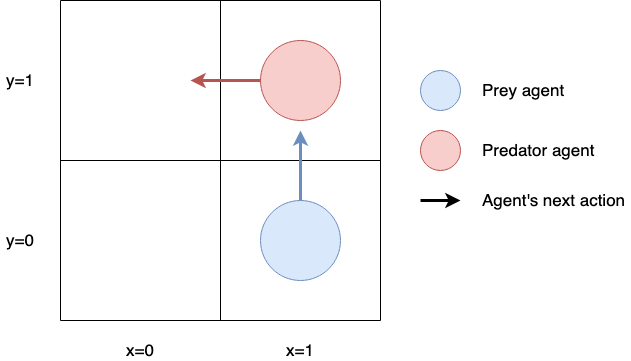
\includegraphics[scale=0.5]{figs/AB-MCMC-1}
	}
	\caption{A simple predator-prey example.\label{fig:AB-MCMC-1}}
\end{figure}

Let a model timestep consist of a matrix $E$ whose elements $e_{\psi a}$ are the number of agents in state $\psi$ that perform act $a$ in this timestep. Note that this matrix will generally be sparse. For example, the timestep shown in Figure~\ref{fig:AB-MCMC-1} would be
\[
E = \kbordermatrix{
	& a_0 & a_1 & a_2 & a_3 & a_4 & a_5 \\
	\psi_0 & 0 & 0 & 0 & 0 & 0 & 0 \\
	\psi_1 & 0 & 0 & 1 & 0 & 0 & 0 \\
	\psi_2 & 0  & 0 & 0 & 0 & 0 & 0 \\
	\psi_3 & 0 & 0 & 0 & 0 & 0 & 0 \\
	\psi_4 & 0  & 0 & 0 & 0 & 0 & 0 \\
	\psi_5 & 0 & 0 & 0 & 0 & 0 & 0 \\
	\psi_6 & 0 & 0 & 0 & 0 & 0 & 0 \\
	\psi_7 & 1 & 0 & 0 & 0 & 0 & 0 \\ 
}
\]
where all elements are zero except those representing agent $\psi_1$ performing action $a_2$ and agent $\psi_7$ performing action $a_0$.

Finally, let a model trajectory be a tensor, $T$, consisting of a number of model timesteps. ie. a slice of $T$, $T^t$, is the timestep matrix for time $t$, and an element of $T$, $T^t_{\psi a}$, is the number of agents in state $\psi$ that perform act $a$ in timestep $t$.

The timestep function for a predator/prey agent is shown in algorithm \ref{agentTimestep} (where we assume the grid has periodic boundary conditions).

\begin{algorithm}
	\caption{Timestep of a predator/prey agent}
	\label{agentTimestep}
	\begin{algorithmic}
		\Function{Timestep}{agent, otherAgents}
		\If{agent.isaPredator}
		\If{\Call{random}{ } < $\beta_0$ and number of prey on neighbouring gridsquares of otherAgents > 0}
		\State\Return give-birth \Comment{more likely to reproduce when food is available}
		\EndIf
		\If{\Call{random}{ } < $\gamma_0$}
		\State\Return die
		\EndIf
		\Else
		\If{\Call{random}{ } < $\beta_1$}
		\State\Return give-birth
		\EndIf
		\If{\Call{random}{ } < $\gamma_1$}
		\State\Return die
		\EndIf
		\If{\Call{random}{ } < $\delta$ and number of predators on this or neighbouring gridsquares of otherAgents > 0}
		\State\Return die \Comment{been eaten by predator}
		\EndIf
		
		\EndIf
		\State \Return move-left, move-right, move-up or move-down based on a call to \Call{Random}{ }
		\EndFunction
	\end{algorithmic}
\end{algorithm}

\subsection{The posterior}
A trajectory must satisfy a number of constraints in order to be a possible trajectory of an ABM. Since the elements of a trajectory are counts, they must all be non-negative integers, we'll call this the \textit{non-negative integer constraint}
\begin{equation}
\forall t,\psi, a: T^t_{\psi a} \ge 0, T^t_{\psi a} \in \mathbb{Z}
\label{nonNegativeInt}
\end{equation}

A trajectory, $T^t_{\psi a}$, must also be \textit{continuous} which means that the number of agents in each state at the end of timestep $t-1$ must be the number of agents in each state at the beginning of timestep $t$. This can be expressed in terms of the \textit{continuity constraints}:
\begin{equation}
\forall t \in 1 ... n:\forall \phi: \sum_{\psi, a} F(\psi, a)_\phi T^{t-1}_{\psi a} - \sum_a T^t_{\phi a} = 0
\label{continuous}
\end{equation}
where the trajectory runs from $t=0$ to $t=n$. If a trajectory satisfies constraints \ref{nonNegativeInt} and \ref{continuous} we say that it is \textit{valid}.

If we let $\Psi^t_\psi$ be the number of agents in state $\psi$ at the beginning of timestep $t$ then the prior probability of a trajectory is
\[
P(T) =
\begin{cases}
P\left(\Psi^0_{*} = \sum_a T^0_{* a}\right) \prod_{\psi, t} P\left(T^t_{\psi *} \mid \Psi^t_* = \sum_a T^t_{* a}\right) & \text{if } T \text{ is valid} \\
0 & \text{otherwise}
\end{cases}
\]
where $P(\Psi^0_*)$ is our prior beliefs about the state at time $t=0$, and we use $*$ as an index when we want to emphasise that the index remains unbound.

For example, in the predator/prey model, we may know the probability of finding a predator or prey at each gridpoint at $t=0$, may not know the exact positions of each agent so the prior would be a product of Poisson distributions
\[
P(\Psi^0_*) = \prod_\psi \frac{\lambda_\psi^{\Psi^0_\psi} e^{\lambda_\psi}}{\Psi^0_\psi!}.
\]

However, we know the probability that a single agent in a given state will perform an action given the state of the other agents, this is defined by the agent timestep function, so the joint probability that $\Psi^t_\psi$ agents will perform actions $T^t_{\psi *}$ is the multinomial distribution
\[
P\left(T^t_{\psi *} \mid \Psi^t_*\right) = \Psi^t_\psi!\prod_a \frac{P(\pi(\psi,\Psi^t_*)=a)^{T^{t}_{\psi a}}}{T^{t}_{\psi a}!}.
\]
So the prior probability of a trajectory is
\[
P(T) =
\begin{cases}
P(\Psi^0_* = \sum_aT^0_{* a}) \prod_{t, \psi}\left(\sum_a T^t_{\psi a}\right)!\prod_a \frac{P(\pi(\psi,\sum_bT^{t}_{\phi b})=a)^{T^{t}_{\psi a}}}{T^{t}_{\psi a}!} & \text{if } T^t_{\psi a} \text{ is valid} \\
0 & \text{otherwise}\\
\end{cases}
\]

Suppose we also have a set of noisy, aggregate observations, $\Omega$, that have a likelihood function $P(\Omega|T^t_{\psi a})$. In our running example, let's suppose we periodically note down when and where we see footprints of predator and prey. Our aim is to generate a number of samples from the posterior distribution
\[
P(T^t_{\psi a}|\Omega) \propto P\left(\Omega \middle| T^{t}_{\psi a}\right)P(T^t_{\psi a})
\]

We assume that observations are independent given the trajectory and that each individual observation in $\Omega$ can be simulated by a computer program $\omega(T^t_{\psi a})$ which may make calls to a random number generator. The probability, $P(\omega(T^t_{\psi a}) = v)$, that the program returns a value $v$ defines the likelihood of observing value $v$ upon making observation $\omega$ on trajectory $T^t_{\psi a}$. i.e. $\omega(T^t_{\psi a})$ is just a simulation of the observation, which is usually quite easy to express as a computer program and to compute. 

In the case of the predator prey model, let's suppose that at the end of every day we go out to a fixed set of inspection sites and check for footprints. Suppose that if predators were present in the grid-square containing an inspection site on that day, there's a 50\% chance we'll see a footprint, and if prey were present, there's a 25\% chance. The observation function for a site is shown in algorithm \ref{observationFunc}

\begin{algorithm}
	\caption{Function for observing predator/prey footprints at a site}
	\label{observationFunc}
	\begin{algorithmic}
		\Function{ObserveFootprints}{T} \Comment{T is the ABM trajectory}
		\State $t \leftarrow$ time of observation
		\State $x \leftarrow$ x-position of observation
		\State $y \leftarrow$ y-position of observation
		\State $G \leftarrow$ size of grid
		\State $\psi \leftarrow G^2 + Gy + x$   \Comment{state of predator in this gridsquare}  
		\State $\phi \leftarrow Gy + x$     \Comment{state of prey in this gridsquare}
		\State $F_{pred} \leftarrow$ \Call{False}{}  \Comment{did we observe predator footprints?}
		\State $F_{prey} \leftarrow$ \Call{False}{}  \Comment{did we observe prey footprints?}
		
		\If{$\sum_a T^t_{\psi a} > 0$ and \Call{Random}{ } < 0.5}
		\State $F_{pred} \leftarrow$ \Call{True}{}
		\EndIf
		\If{$\sum_a T^t_{\phi a} > 0$ and \Call{Random}{ } < 0.25}
		\State $F_{prey} \leftarrow$ \Call{True}{}
		\EndIf
		\State\Return $F_{pred}$, $F_{prey}$
		\EndFunction
	\end{algorithmic}
\end{algorithm}


Given this
\[
P(\Omega|T^t_{\psi a}) = \prod_{(\omega,v) \in \Omega} P(\omega(T^t_{\psi a})=v)
\]

Also, for notational convenience, and without loss of generality, we express our prior beliefs in terms of a set of observations, $\Omega_0$, at $t=0$, so that $P_0(\sum_a T^0_{\psi a}) \propto \prod_{(\omega,v) \in \Omega_0} P(\omega(T^t_{\psi a})=v)$ (this also allows any priors that aren't at $t=0$). The posterior can now be written as
\begin{equation}
P(T^t_{\psi a}|\Omega) \propto 
\begin{cases}
\prod_{(\omega,v) \in \Omega} P\left(\omega(T^{t}_{\psi a})=v\right) \prod_{t, \psi}\left(\sum_a T^t_{\psi a}\right)!\prod_{a}\frac{P(\pi(\psi,\sum_bT^{t}_{\phi b})=a)^{T^{t}_{\psi a}}}{T^t_{\psi a}!} & \text{if } T^t_{\psi a} \text{ is valid} \\
0 & \text{otherwise}\\
\end{cases}
\label{posterior}
\end{equation}
where $\Omega$ now includes any priors.

In many practical applications, sampling from this posterior is difficult because it has zero probability for the vast majority of trajectories (i.e. most trajectories are invalid, contain an impossible action or are refuted by the observations). This is true of our predator/prey model, for example. Even though we can generate valid trajectories that fit the prior by simply performing a forward execution of the model from an initial state drawn from the prior, if the trajectory has no predator or prey at a time and place that we observed footprints, then the observations refute the trajectory and the probability falls to zero. It doesn't take many observations until the probability of randomly choosing a trajectory that fits the observations becomes very small indeed. So simple techniques such as rejection sampling are not practical.

In this paper we'll use the Metropolis-Hastings algorithm to generate samples. However, this method requires a proposal function which randomly generates the next sample given the current one. However, given the current sample, we still have the problem of finding a trajectory with non-zero probability. For example if we generate a new trajectory by perturbing one or more elements of the last sample at random (a common strategy with Metropolis-Hastings), it's very unlikely that we'll end up with a trajectory that is valid, contains only possible actions and satisfies the observations. So, the proposed next sample would almost certainly be rejected and we'd probably end up stuck on the first sample until we grew old.

\section{Approximating the support of the posterior}
%##########################################


To solve this problem we'd like to constrain our proposal function to the support of the posterior, $\supp(P(T^t_{\psi a}|\Omega))$ (i.e. the set of trajectories that have non-zero probability).

If we let
\[
\pi'(s, \xi, T^t_{\psi a}) = \pi(\xi,\sum_bT^{s}_{\phi b})
\]
Then from equation \ref{posterior}
\begin{equation}
\supp (P( \,.\, |\Omega)) = 
\bigcap_{(\omega,v) \in \Omega}  \supp\left(P\left(\omega(.)=v\right)\right) \cap
\bigcap_{t, \psi, a} \left(\supp\left(P\left( \pi'(t,\psi,.) = a \right)\right) \cup \left\{T^s_{\xi b}: T^t_{\psi a} = 0\right\}\right) \cap
\left\{T^t_{\psi a} \mid T^t_{\psi a} \text{is valid}\right\}
\label{support}
\end{equation}
i.e. in order for the posterior to be non-zero, all the observation likelihoods must be non-zero, the probability of each agent's action at every timestep must be non-zero and the trajectory must be valid (note that we've dropped the exponent in the agent action term as it doesn't affect the support).

The first two terms in equation \ref{support} consists of the supports of computer programs whose inputs are ABM trajectories and whose outputs are given, i.e. the set of trajectories that, when passed to a computer program, would produce a given output.

Calculating the support of a computer program for a given output is, in full generality, NP-complete\footnote{Consider, for example, a program that accepts an assignment of variables to truth values, and returns true if that assignment satisfies a Boolean formula. Deciding whether the support of this program, given that it returns true, is empty or not is equivalent to solving the Boolean satisfiability problem, which is known to be NP-complete\cite{cook1971complexity}} but it is possible to use a technique known as \textit{abstract interpretation}\cite{cousot1977abstract} to efficiently calculate a superset of the support. So, given a computer program $\rho$, we can calculate a set $\mathcal{P}(\rho, v)$ such that
\[
\supp(P(\rho(.)=y)) \subset \mathcal{P}(\rho, v)
\]
Tools to perform abstract interpretation already exist (e.g. PAGAI\cite{henry2012pagai}) and are used widely in applications such as the verification of safety critical systems\cite{blanchet2003static} and in practice $\mathcal{P}(\rho, v)$ is often reasonably tight (i.e. most members of $\mathcal{P}(\rho, v)$ are in $\supp(P(\rho(.)=y))$). For our application we choose to express $\mathcal{P}(\rho, v)$ in terms of a set of linear inequalities on $\rho$'s inputs, this corresponds to the abstract domain of convex polyhedra\cite{cousot1978automatic}\cite{becchi2018efficient}. Calls to the random number generator can be dealt with in the abstract domain by generating a new variable, $r$, that satisfies $0 \le r < 1$ for each call to \texttt{Random()}. These can either be left in as ``auxiliary'' variables in the same way as slack variables, or removed as soon as the variable goes out of scope by finding the convex hull of the projection into a lower dimensional space (this can be done using the double description method\cite{motzkin1953double}).

If we replace the supports in equation \ref{support} with their equivalent supersets we end up with a superset of the posterior
\begin{equation}
\supp(P(.|\Omega)) \subset
\bigcap_{(\omega,v) \in \Omega}  \mathcal{P}(\omega, v) \cap
\bigcap_{t, \psi, a} \left( \mathcal{P}(\pi'(t,\psi,.), a) \cup \left\{T^s_{\xi b}: T^t_{\psi a} = 0\right\} \right)\cap
\left\{T^t_{\psi a} \mid T^t_{\psi a} \text{is valid}\right\}
\label{linearSupport}
\end{equation}

Constraining our proposal function to members of the superset in equation \ref{linearSupport} instead of the true support won't affect the stationary distribution of the Markov Chain. If the proposal function happens to return a trajectory that isn't in $\supp(P(\rho(.)=y))$ then it will just be rejected. This is fine as long as we generate acceptable proposals at a reasonable rate.

The final term in equation \ref{linearSupport}, which requires the trajectories in the support to be valid, consists of the continuity constraints of equation \ref{continuous}, which are also linear constraints so can be treated along with the other constraints, and the non-negative integer constraints of equation \ref{nonNegativeInt} which we leave as separate constraints.

The union term in equation \ref{linearSupport} can also be transformed to a set of linear constraints, but the way we do this depends on the type of ABM we're dealing with, so we defer the explanation until sections \ref{Fermionic} and ...

Without loss of generality, we express inequalities as equalities by introducing slack variables so that
\[
\sum_i c_i x_i \le y
\]
is equivalent to
\[
\begin{split}
\sum_i c_i x_i + \lambda & = y \\
\text{subject to}\ \lambda & \ge 0 \\
\end{split}
\]

All the constraints can now be gathered into a standard matrix form
\begin{equation}
\begin{split}
AX &= B \\
\text{subject to}\ x_i &\ge 0\\
x_i &\in \mathbb{Z}
\end{split}
\label{Axy}
\end{equation}
where the vector $X$ contains the elements of the trajectory tensor $T^t_{\psi a}$ and the slack variables $\lambda$.

\section{From convex polyhedron to Markov process}
%#####################################################

Given a set of inequalities that contain the support of the posterior, we next need to define a stochastic proposal function $f:\mathbb{S} \to \mathbb{S}$ on a set of Markov states, $\mathbb{S}$, where each state, $S$, is associated with a trajectory $T(S)$. The proposal function should have the following properties:
\begin{itemize}
	\item There should be a set of transitions with non-zero probability between any two Markov states. This ensures proper mixing as time tends to infinity.
	
	\item At the stationary point, the probability of being in a state associated with trajectory $T$ should be our target posterior probability $P(T \mid \Omega)$.
	
	\item For any transition from state $S_a \to S_b$ the probability of transitioning from $S_b \to S_a$ should be non-zero. This allows us to attain detailed balance by using the Metropolis Hastings algorithm.
	
	\item The proposal function should be computationally efficient. 
\end{itemize}

\subsection{A proposal function for a Fermionic ABM}
\label{Fermionic}
%#############################################

We define a Fermionic ABM to be one where no two agents can share the same state at the same time. i.e. in addition to the validity constraints of equations \ref{nonNegativeInt} and \ref{continuous} the trajectory of a Fermionic ABM also satisfies the \textit{Fermionic constraint}
\begin{equation}
\begin{split}
\forall t,\psi: \sum_a T^t_{\psi a} \le 1 \\
\forall \phi: \sum_{\psi, a} F(\psi, a)_\phi T^n_{\psi a} \le 1
\end{split}
\label{fermionic}
\end{equation}
in which case we call it a \textit{Fermionic trajectory} [this can be weakened to $T^t_{\psi a} \le 1$].

It is clear that every element of a Fermionic trajectory must be either 0 or 1. This means we can easily convert the union term in equation \ref{linearSupport} 
\[
\mathcal{P}(\pi'(t,\psi,.), a) \cup \left\{T^s_{\xi b}: T^t_{\psi a} = 0\right\}
\]
into a set of linear constraints. Expanding $\mathcal{P}$ we have
\[
\left(\bigcap_j \sum_i a_{ij}x_i \le b_j \right) \cup \left\{X: x_k = 0\right\} = \bigcap_j \left( \sum_i a_{ij}x_i \le b_j  \cup \left\{X: x_k = 0\right\}\right)
\]
where we've projected the elements of the trajectory $T^t_{\psi a}$ into a vector $X$. But
\[
\sum_i a_{ij}x_i \le b_j  \cup \left\{X: x_k = 0\right\} = \sum_i a_{ij}x_i + \left(\sum_i \frac{|a_{ij}| + a_{ij}}{2} - b_j\right)x_k \le \sum_i \frac{|a_{ij}| + a_{ij}}{2} 
\]
since all $x_i$ are also either 0 or 1 so $\sum_i a_{ij}x_i$ must be less than $\frac{|a_{ij}| + a_{ij}}{2}$ and the constraint is satisfied if $x_k$ is 0, whereas we have the original constraint if $x_k$ is 1.

So, taking our predator prey agent of algorithm \ref{agentTimestep} as an example, we can see that the move, reproduce and die actions can be returned irrespective of the state of other agents\footnote{the Fermionic constraint is dealt with separately, so we don't need to worry about that here}, so for these actions the union is also unconditionally true. However, the reproduction actions of a predator are conditional on there being some prey on neighbouring gridsquares. So, suppose we have a predator in state $\psi$ at time $t$, the support of it's timestep function given that it returns a reproduction action is
\[
\sum_{i \in N^t_\psi} -x_i \le -1
\]
where $N^t_\psi$ is the set of indices that correspond to elements of $T^t_{\phi a}$ where $\phi$ is a prey on a gridsquare neighbouring $\psi$ at time $t$. So, taking the union with $\left\{X: x_k = 0\right\}$, the final constraint for a predator in state $\psi$ at time $t$ is
\[
\sum_{i \in N^t_\psi} -x_i  + x_k  \le 0
\]

\begin{theorem}
	All trajectories that satisfy equations \ref{nonNegativeInt} and \ref{fermionic} are at extreme points. Where an extreme point is one that can't be expressed as a linear combination of two other points that satisfy the constraints.
\end{theorem}
\begin{proof}
	
	Inequality \ref{fermionic} can only be satisfied by non-negative integers if, for any given $t$ and $\psi$ either all $T^t_{\psi a}$ are zero or one element of $T^t_{\psi a}$ is one and the rest zero. In the first case the solution is touching all $|a|$ of the $T^t_{\psi a} \ge 0$ constraints, in the second case the solution is touching $|a|-1$ of the $T^t_{\psi a} \ge 0$ constraints and one $\sum_a T^t_{\psi a} \le 1$ constraint to give a total of $|a|$.
	
	[Conversely, we can show that all extreme points are integer points, so we have the polytope of integer solutions]
	
	[In the case of the action Fermionic constraint, this can be seen immediately since equations \ref{nonNegativeInt} and the action Fermionic constraint describe a unit hupercube, so all integer solutions are on vertices.]
	
\end{proof}

%\begin{theorem}
%For any pair of valid trajectories, $A$ and $B$, there exists a path along edges of the polyhedron from $A$ to $B$ that only traverses through integer solutions.
%\end{theorem}
%\begin{proof}
%[Take the difference A-B and decompose into integer null vectors (loops)]
%\end{proof}

This seemingly abstract fact has a profound practical consequence for the efficiency of our proposal function.
Given a system of $m$ linear constraints on $n$ variables expressed in the form $AX=B$, let a \textit{pivot state} be a partition of the variables into $m$ \textit{basic variables} and $n-m$ \textit{non-basic variables} so we can express the constraints in the form
\begin{equation}
A_bX_b + A_nX_n = B
\label{tableau1}
\end{equation}
where $X_b$ and $X_n$ are the basic and non-basic variables respectively, $A_b$ is the matrix formed from the columns in $A$ that correspond to the basic variables and $A_n$ is the matrix formed from the columns of $A$ that correspond to the non-basic variables. If we now constrain all non-basic variables to zero then we're left with $A_bX_b = B$ but since $A_b$ is an $m \times m$ square matrix then $X_b = A_b^{-1}B$ gives a unique solution, as long as $A_b$ is invertable. If $A_b$ is invertable and $X_b$ has no negative entries then we say that the pivot state is valid. It can be shown that all valid pivot states of equations \ref{Axy} correspond to extreme points\cite{dantzig1955generalized}.

This idea leads to a computationally very efficient way of perturbing trajectories. We begin by representing the constraints and the current trajectory in the form of equation \ref{tableau1}. If we multiply any row of $A_b$ by some constant, $c$, then the truth of equation \ref{tableau1} can be maintained by multiplying the same row of $A_n$ and of $B$ by $c$ as well. Similarly if we add one row of $A_b$ to another row, the equations can be maintained by performing the same row operation on $A_n$ and $B$. If the pivot state is valid, then $A_b$ is invertable so we can use Gaussian elimination, by performing a sequence of row additions and multiplications, to transform $A_b$ into a form such that each row and column is zero on all elements except one, which is 1. We'll call this the standard form. Once in this form, if we assume $X_n = 0$ the solution for $X_b$ can be read off directly from $B$.

Given a valid pivot state in standard form, a perturbed valid solution can be generated by choosing a column, $C$, of $A_n$, with at least one positive-valued row, and choosing from among those rows the one, $C_i$, that minimises $B_i/C_i$. We then make the variable corresponding to column $C$ a basic variable and make the basic variable corresponding to row $i$ of $A_b$ non-basic by swapping column $C$ with the column on row $i$ of $A_b$ that has value 1. $A_b$ is now not in standard form as column $C$ will, in general, have more than one non-zero value so we perform Gaussian elimination (row additions and multiplications) to return it to standard form. This perturbation is known as a \textit{pivot} operation and is the same method as employed in the Simplex algorithm\cite{dantzig1955generalized}\cite{vanderbei2015linear}. This is exactly what we need for our proposal function since it efficiently generates a new valid trajectory from a current one.

\subsubsection{Fractional solutions and feasibility pumps}
%#########################################################

Although pivoting ensures solutions are positive, there may exist extreme points that don't fall on the grid of integer solutions and so do not satisfy the integer constraint. However, if we posit the existence of a \textit{null trajectory} and associate all fractional solutions with the null trajectory, then simply ignore null samples, then we end up with samples from the posterior, as required (i.e. the Markov chain can pass through fractional states, but no sample is generated when doing so). However, we don't want to spend too much computational effort moving between fractional states without generating samples, so we encourage the Markov process away from these fractional states using a \textit{feasibility pump} which works in the following way: [Score pivots from a fractional state by sum of difference between integer rounding of this state and pivoted state (no update of target integer solution), and by difference between integer rounding of pivoted state and pivoted state and the difference between the integer roundings of this and pivoted state (target integer solution updated). ]

%by multiplying their probability by a ``fractional penalty'' $e^{-kn}$ where $n$ is the number of non-integer values in the solution and $k$ is a constant parameter [better to use a stochastic extension of Fischetti(2005) feasibility pump here. Fractional solutions are ``augmented'' with an integer, infeasible(negative) solution which also changes stochastically].

\subsubsection{Dealing with degeneracy}
%######################################

The use of pivoting is complicated somewhat when the solutions are degenerate. A degenerate solution is one that can be generated by more than one pivot state. This can occur when a pivot state has basic variables with value zero (in which case we say the pivot state is degenerate and call the zero variables \textit{degenerate varaibles} of the pivot state). Pivoting on a degenerate variable does not change the solution since during a pivot the outgoing basic variable becomes constrained to zero; but if the basic-variable's value was zero to start with, constraining it to zero has no effect on the solution (for a thorough theoretical development of degeneracy see \cite{zornig93degeneracy}). This is problematic because we need to assign a probability to each Markov state but under degeneracy a pivot state can't be given the probability of its trajectory because this would result in degenerate trajectories being ``counted'' multiple times, once for each degenerate pivot state of the trajectory. To maintain the correct distribution, the probabilities of all the degenerate pivot states of a given trajectory should sum to the probability of that trajectory.

To solve this problem in a computationally efficient way we introduce the concept of an \textit{ordered pivot state} which consists of a partition of the variables into basic and non-basic variables as before, but in addition there is now an ordering of the basic variables. Since we represent $A_b$ as a matrix in our standard form representation, it is easy to represent this ordering in the ordering of the rows of $A_b$. As before, the validity of equation \ref{tableau1} can be maintained under permutations of the ordering of the rows of $A_b$ by performing the same row permutations on $A_n$ and $B$. We now associate a Markov state with each ordered pivot state, assigning it a probability according to algorithm \ref{probAlgorithm}:

\begin{algorithm}
	\caption{Algorithm to calculate probability of an ordered pivot state}
	\label{probAlgorithm}
	\begin{algorithmic}
		\Function{Probability}{$A_b$,$A_n$,$B$} \Comment{Standard representation of an ordered pivot state}
		\State $P_T \leftarrow$ the probability of the trajectory of the current solution
		\State $P_d \leftarrow 1.0$
		\State $C \leftarrow \emptyset$
		\State $r \leftarrow 0$
		\For{$i = |B|-1 \text{ down to } 0$}
		\If{B[i] == 0}
		\State $C \leftarrow C \ \cup $ the indices of the non-zero entries in row $i$ of $A_n$
		\State $P_d \leftarrow P_d/(|C|+r+1)$
		\State $r \leftarrow r + 1$
		\EndIf
		\EndFor
		\State \Return $\frac{P_d P_T\sigma!}{|B|!}$
		\EndFunction
	\end{algorithmic}
\end{algorithm}

The proposal function for ordered pivot states is shown in algorithm \ref{proposal}

\begin{algorithm}
	\caption{Proposal function for ordered pivot states}
	\label{proposal}
	\begin{algorithmic}
		\Function{Proposal}{$A_b$, $A_n$, $B$} \Comment{Standard representation of the current ordered pivot state}
		\State $A_b',A_n',B' \leftarrow A_b,A_n,B$
		\State $\alpha, \beta \leftarrow$ constant parameters
		\State $p_0 \leftarrow$ the set of degenerate pivots of $(A_b,A_n,B)$ (i.e. the ones that do not change the solution)
		\State $p_1 \leftarrow$ the set of non-degenerate pivots of $(A_b,A_n,B)$ (i.e. the ones that change the solution)
		\State $P_{f/b} \leftarrow 1$ \Comment{the ratio of probabilities of making this transition forwards/backwards}
		\If{\Call{Bernoulli}{$\alpha$}}
		\State $r \leftarrow$ choose member of $p_1$ with uniform probability
		\State perform pivot $r$ on $(A_b',A_n',B')$
		\State $p'_1 \leftarrow $ number of non-degenerate pivots of $(A_b',A_n',B')$
		\State $P_{f/b} \leftarrow \frac{|p'_1|}{|p_1|}$
		\ElsIf{\Call{Bernoulli}{$\beta$}}
		\State $r \leftarrow$ choose member of $p_0$ with uniform probability
		\State perform pivot $r$ on $(A_b',A_n',B')$
		\State $p'_0 \leftarrow $ number of degenerate pivots of $(A_b',A_n',B')$
		\State $P_{f/b} \leftarrow \frac{|p'_0|}{|p_0|}$
		\Else
		\State choose two rows $a$ and $b$ with uniform probability
		\State swap rows $a$ and $b$ of $(A_b',A_n',B')$
		\EndIf
		\State \Return $(A_b',A_n',B',P_{f/b})$
		\EndFunction
	\end{algorithmic}
\end{algorithm}



We now show that this assignment of probability to ordered pivot states has the property that the sum of the probabilities of ordered pivot states associated with a trajecotry is the probability of that trajectory.

First some notation: let $\mathbb{E}(T)$ be the set of all ordered pivot states with solution $T$, let $T(S)$ be the trajectory associated with pivot state $S$, let $D(S)$ be the tuple of degenerate variables in ordered pivot state $S$, let $D_{\le n}(S)$ be the n-tuple consisting of the first $n$ elements of $D(S)$ and let
\begin{equation}
C(\mathbb{S} \mid V) = \left\|\left\{ V^+ :  S \in \mathbb{S}, V^+ = D_{\le |V|+1}(S), V^+_{\le |V|}=V \right\}\right\|
\label{count}
\end{equation}
i.e. among the members of $\mathbb{S}$ that have the degenerate variable prefix $V$, $C(\mathbb{S}|V)$ counts how many distinct degenerate variable prefixes of length $|V|+1$ there are.




\begin{theorem}
	If we assign the probability
	\begin{equation}
	P(S) =  \frac{\sigma_{T(S)}!}{m!} \frac{P_{T(S)}}{\prod_{q=0}^{\sigma_{T(S)}-1} C(\mathbb{E}(T(S)) \mid D_{\le q}(S))}
	\label{pivotProb}
	\end{equation}
	to pivot state $S$, where $m$ is the number of constraints and $\sigma_{T}$ is the degeneracy of trajectory $T$ (i.e. $m$ minus the number of non-zero variables in $T$) then
	\[
	\sum_{S \in \mathbb{E}(T)} P(S) = P_{T}
	\]
\end{theorem}
\begin{proof}
	Expanding the sum over degenerate states
	\[
	\sum_{S \in \mathbb{E}(T)} P(S) =
	P_T \frac{\sigma_T!}{m!} \sum_{S \in \mathbb{E}(T)} \frac{1}{\prod_{q=0}^{\sigma_T-1} C(\mathbb{E}(T) \mid D_{\le q}(S))}
	\]
	
	Notice first that all pivot states with the same $\sigma_T$-tuple of degenerate variables, $D(S)$, have the same probability. There are exactly $\frac{m!}{\sigma_T!}$ ordered pivot states with a given $D(S)$, corresponding to the different placings of the $m-\sigma_T$ non-degenerate basic variables among the $m$ possible positions. So, if we let
	\[
	\mathbb{D}(T) = \left\{ D(S) : S \in \mathbb{E}(T) \right\}
	\]
	then
	\[
	\sum_{S \in \mathbb{E}(T)} P(S) = P_T \sum_{D \in \mathbb{D}(T)} \frac{1}{\prod_{q=0}^{\sigma_T-1} C(\mathbb{E}(T) \mid D_{\le q})}
	\]
	Since $C(\mathbb{S} \mid V)$ depends only on the order of the degenerate variables in the members of $\mathbb{S}$
	\[
	C(\mathbb{E}(T) \mid V) = C(\mathbb{D}(T) \mid V)
	\]
	so
	\begin{equation}
	\sum_{S \in \mathbb{E}(T)} P(S) = P_T \sum_{D \in \mathbb{D}(T)} \frac{1}{\prod_{q=0}^{\sigma_T-1} C(\mathbb{D}(T) \mid D_{\le q})}
	\label{normalForm}
	\end{equation}
	if we separate the terms in the sum into groups that share the same prefix apart from the last variable then we get
	\[
	\sum_{S \in \mathbb{E}(T)} P(S) = 
	P_T \sum_{V : D \in \mathbb{D}(T), V = D_{\le (\sigma_T-1)}} 
	\left(
	\frac{1}{\prod_{q=0}^{\sigma_T-2} C(\mathbb{D}(T|V_{\le q}))}
	\sum_{V^+: V^+ \in \mathbb{D}(T), V = V^+_{\le (\sigma_T-1)}}
	\frac{1}{C(\mathbb{D}(T|V))}
	\right)
	\]
	So
	\[
	\sum_{S \in \mathbb{E}(T)} P(S) = 
	P_T \sum_{V : D \in \mathbb{D}(T), V = D_{\le (\sigma_T-1)}} 
	\frac{1}{\prod_{q=0}^{\sigma_T-2} C(\mathbb{D}(T|V_{\le q}))}
	\frac{\left\|\left\{V^+: V^+ \in \mathbb{D}(T), V = V^+_{\le (\sigma_T-1)}\right\}\right\|}{C(\mathbb{D}(T|V_{\le (\sigma_T-1)}))}
	\]
	but the final fraction here is 1 by equation \ref{count}, so
	\[
	\sum_{S \in \mathbb{E}(T)} P(S) = 
	P_T \sum_{V : D \in \mathbb{D}(T), V = D_{\le (\sigma_T-1)}} 
	\frac{1}{\prod_{q=0}^{\sigma_T-2} C(\mathbb{D}(T|V_{\le q}))}
	\]
	we can now use the same argument again to reduce the upper bound of $q$ iteratively until we show that the sum on the right hand equals one, so
	\[
	\sum_{S \in \mathbb{E}(T)} P(S) = P_T
	\]
\end{proof}

\begin{theorem}
	Algorithm \ref{probAlgorithm} assigns a probability
	\[
	P(S) =  \frac{\sigma_{T(S)}!}{m!} \frac{P_{T(S)}}{\prod_{q=0}^{\sigma_{T(S)}-1} C(\mathbb{E}(T(S)) \mid D_{\le q}(S))}
	\]
	to pivot state $S$
\end{theorem}
\begin{proof}
	By inspection of the algorithm, it can be seen that the algorithm assigns probability 
	\[
	P(S) =  \frac{\sigma_{T(S)}!}{m!} \frac{P_{T(S)}}{\prod_{r=0}^{\sigma_{T(S)}-1} \left(\left\|C'(S, r)\right\| + r + 1\right)}
	\]
	where
	\[
	C'(S,r) = C'(S,r-1) \cup N(S,r)
	\]
	\[
	C'(S,-1) = \emptyset
	\]
	and $N(S,r)$ is the set of indices of the non-zero entries in the $r$-from-last degenerate row of $A_n$. So, $C'(S,r)$ is the set of columns that have at least one non-zero entry on a degenerate row on or below the $r$-from-last.
	
	However, $C(\mathbb{E}(T(S)) \mid D_{\le q}(S))$ is, by definition, the number of different degenerate variables that can take the $(q+1)^{th}$ place in the list of degenerate variables, given that the first $q$ are given by $D_{\le q}(S)$.
	
	Now, given an ordered pivot state, $S$ in standard form; if there exists a column, $j$, with a non-zero entry in a degenerate row, $i$,  of $A_n$ or $A_b$ below the $q^{th}$ degenerate row, then we can generate a valid member of $\mathbb{E}(T(S))$ with $j$ the $(q+1)^{th}$ variable by pivoting on column $j$ and row $i$ (if not already pivoted in), then swapping row $i$ with whichever row makes it the $(q+1)^{th}$ degenerate variable. Conversely, if there exists a member of $\mathbb{E}(T(S))$ with $j$ as the $(q+1)^{th}$ variable, it must be possible to pivot on the $j^{th}$ column without pivoting out any of the first $q$ degenerate variables or the non-degenerate variables. The only way this is possible is if there is either a non-zero entry in the $j^{th}$ column of $A_n$ or $A_b$ below the $q^{th}$ degenerate row. So, the set of degenerate variables that can take the $(q+1)^{th}$ place is the set of columns that have non-zero entries in degenerate rows below the $q^{th}$ in $A_n$ or $A_b$. From the form of $A_b$ we know immediately that there are $r+1$ columns with non-zero degenerate entries on or below the $r$-to-last degenerate row. So
	\[
	C(\mathbb{E}(T(S)) \mid D_{\le \sigma_{T(S)} -1 - r}(S)) = \left\|C'(S, r)\right\| + r + 1
	\]
	
	
\end{proof}

\subsubsection{Metropolis-Hastings on ordered pivot states}

All this can now be assembled into a sampling algorithm based on Metropolis-Hastings. Starting with the constraints in the form of equation \ref{Axy}, recursively choose a non-zero element on an un-pivoted row and pivot on that element, until we reach an ordered pivot state. In general, $B$ will contain negative elements which means that the solution will not conform to the non-negative constraint. In order to find an initial positive solution let $I^- = \left\{i: B_i < 0\right\}$ be the set of rows of $B$ that are negative and pivot on the column, $j$, that minimises $\sum_{i\in I^-}A_{ij}$. Repeat until a positive solution is found (or no column has a negative sum, in which case no positive solution exists).

From the initial valid pivot state, $S$, generate a proposal pivot state $S'$ and a transition probability ratio $\frac{P(S\rightarrow S')}{P(S' \rightarrow S)}$ using algorithm \ref{proposal} and accept with probability
\[
\alpha = \frac{P(S')}{P(S)}\frac{P(S'\rightarrow S)}{P(S \rightarrow S')}
\]
where the probability of a pivot state is given by algorithm \ref{probAlgorithm}.

Given this, it's clear that all the necessary properties of the proposal function are fulfilled.

\section{Results}

\section{Conclusion}


%\bibliographystyle{unsrtnat}
%\bibliographystyle{apalike} 
\bibliographystyle{apacite}
\bibliography{references}

\end{document}
